\documentclass{article}
\usepackage[utf8]{inputenc}
\usepackage{geometry}
\usepackage{graphicx}
\usepackage{float}
\usepackage{enumitem}  % Added package for customizing itemize spacing
\usepackage{setspace}  % Added package for customizing line spacing
\usepackage{amsmath}  % for mathematical symbols and expressions
\usepackage{amsfonts}  % for additional mathematical fonts
\usepackage{amssymb}  % for additional mathematical symbols
\usepackage{caption}


\geometry{a4paper, total={5.5in, 7.5in}, left=0.75in, right=0.75in, top=0.75in, bottom=0.75in}
\title{Database Querying}
\author{Ioannis Zacharopoulos (2307)/Dimitrios Tselentis (2325)}

% Custom line spacing
\onehalfspacing

\begin{document}

\maketitle

\section*{Question i}
Count all the offshore entities of the database.


\[ \pi_{\text{{COUNT(*)}}}(\text{{entities\_2307\_2325}}) \]


\begin{figure}[h]
    \centering
    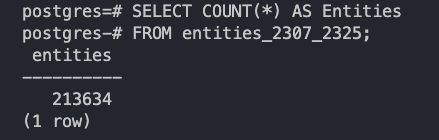
\includegraphics[width=0.6\linewidth]{Q1.png}
    \captionsetup{labelformat=empty}
    \caption{Question 1}
\end{figure}



\newpage

\section*{Question ii}
Find the top-20 countries in terms of the number of officers they have, ordered by this number in descending order.

\begin{figure}[h]
    \centering
    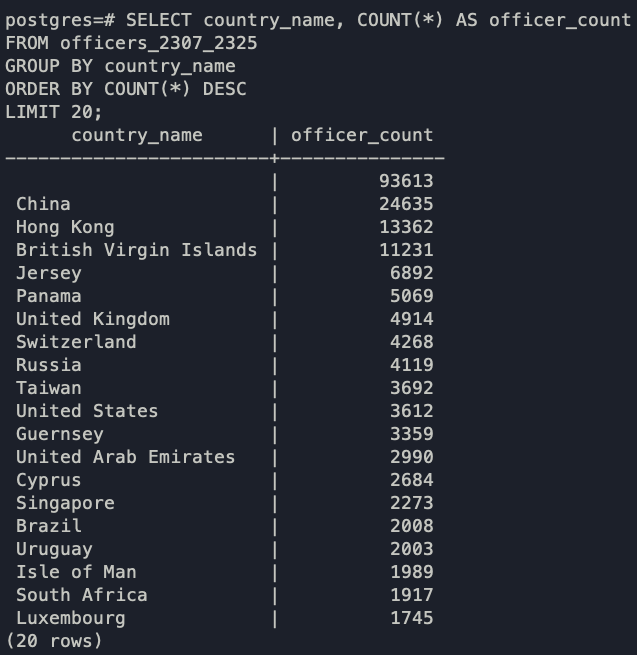
\includegraphics[width=0.9\linewidth]{Q2.png}
    \captionsetup{labelformat=empty}
    \caption{Question 2}
\end{figure}

\newpage

\section*{Question iii}
Find the node\_ids, the names, and the addresses of the officers coming from Greece. For those that there is no registered address, the entry should be returned with the respective attribute empty (NULL).

\[
    \pi_{\text{{o.officer\_id, o.name, a.address}}}(\sigma_{\text{{o.country\_name = 'Greece'}}}) \bowtie_{\text{L}}(\rho_o(\text{{officers\_2307\_2325}}))
\]
\[
    \bowtie_{\text{L}}({\text{{o.officer\_id = oa.officer\_id}}}  (\text{{\(\rho_{\text{{oa}}}(\text{{officers\_addresses\_2307\_2325}})\)}}))
\]
\[
    \bowtie_{\text{L}}({\text{{oa.address\_id = a.address\_id}}}(\rho_{\text{{a}}}(\text{{addresses\_2307\_2325}})))
\]




\begin{figure}[h]
    \centering
    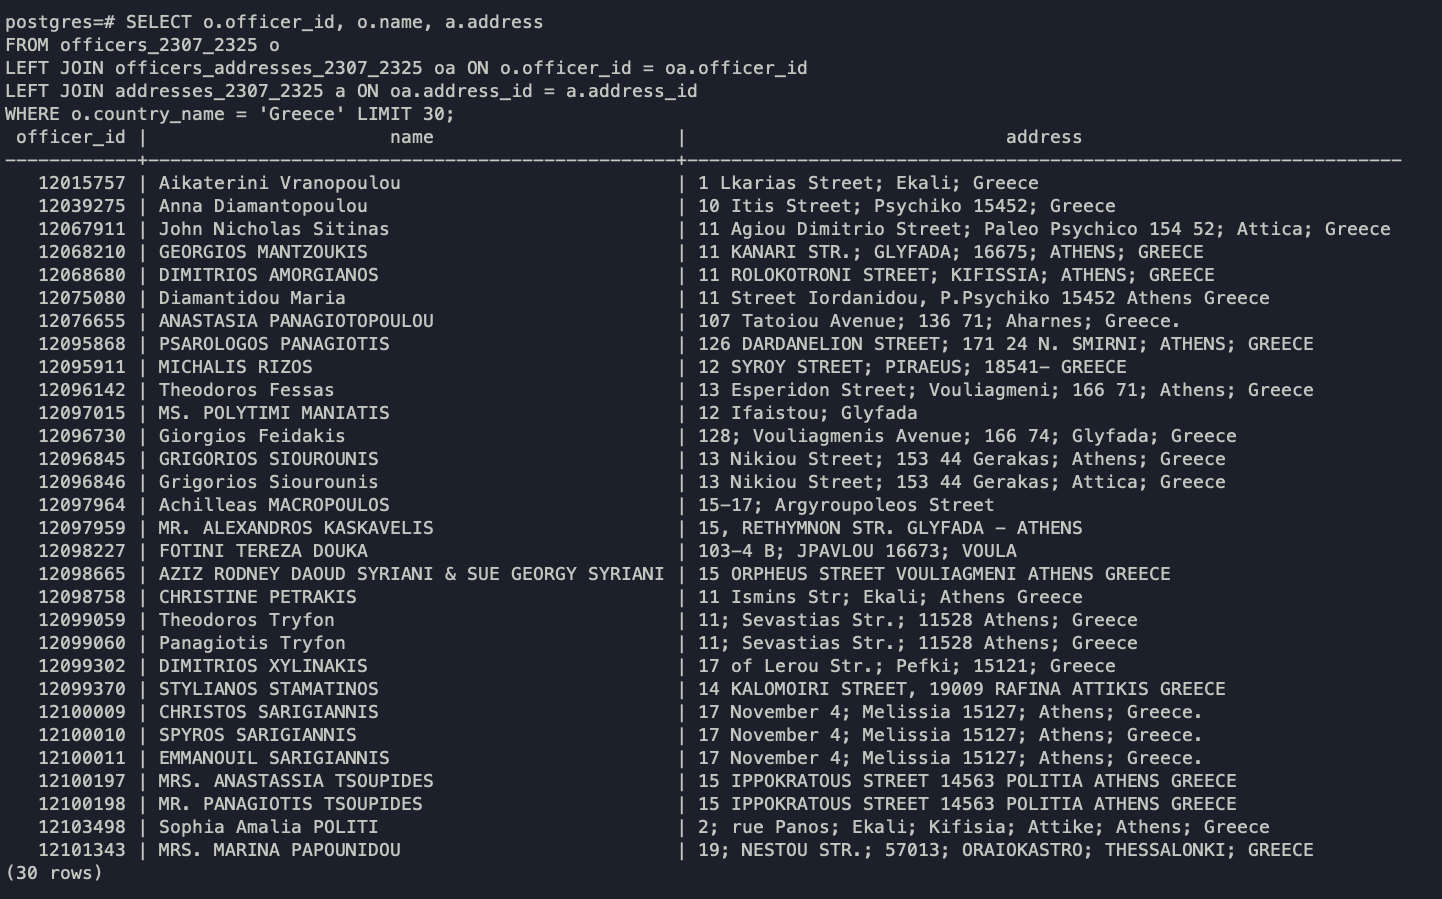
\includegraphics[width=1\linewidth]{Q3.png}
    \captionsetup{labelformat=empty}
    \caption{Question 3: We used limit 30 for abbreviation purposes.}
\end{figure}

\newpage

\section*{Question iv}
Find the node\_ids, the names, and the addresses of all officers who play a role in an offshore entity; this entity’s country should be Greece and its jurisdiction should be in Seychelles. For those officers that there is no registered address, the entry should be returned with the respective attribute empty (NULL).
\[
    \pi_{\text{o.officer\_id, o.name, a.address}}
\]
\[
    \sigma_{\text{e.country\_name = 'Greece' AND e.jurisdiction\_description = 'Seychelles'}}
\]
\[
    \bowtie_{\text{L}}(\rho_o(\text{{officers\_2307\_2325}}))
\]
\[
    \bowtie_{\text{L}}({\text{o.officer\_id = ore.officer\_id}} (\rho_{\text{ore}}(\text{officers\_roles\_entities\_2307\_2325})))
\]
\[
    \bowtie_{\text{L}}({\text{ore.entity\_id = e.entity\_id}}
    (\rho_{\text{oa}}(\text{officers\_addresses\_2307\_2325})))
\]
\[
    \bowtie_{\text{L}}({\text{oa.officer\_id = o.officer\_id}} (\rho_{\text{a}}(\text{addresses\_2307\_2325})))
\]
\begin{figure}[h]
    \centering
    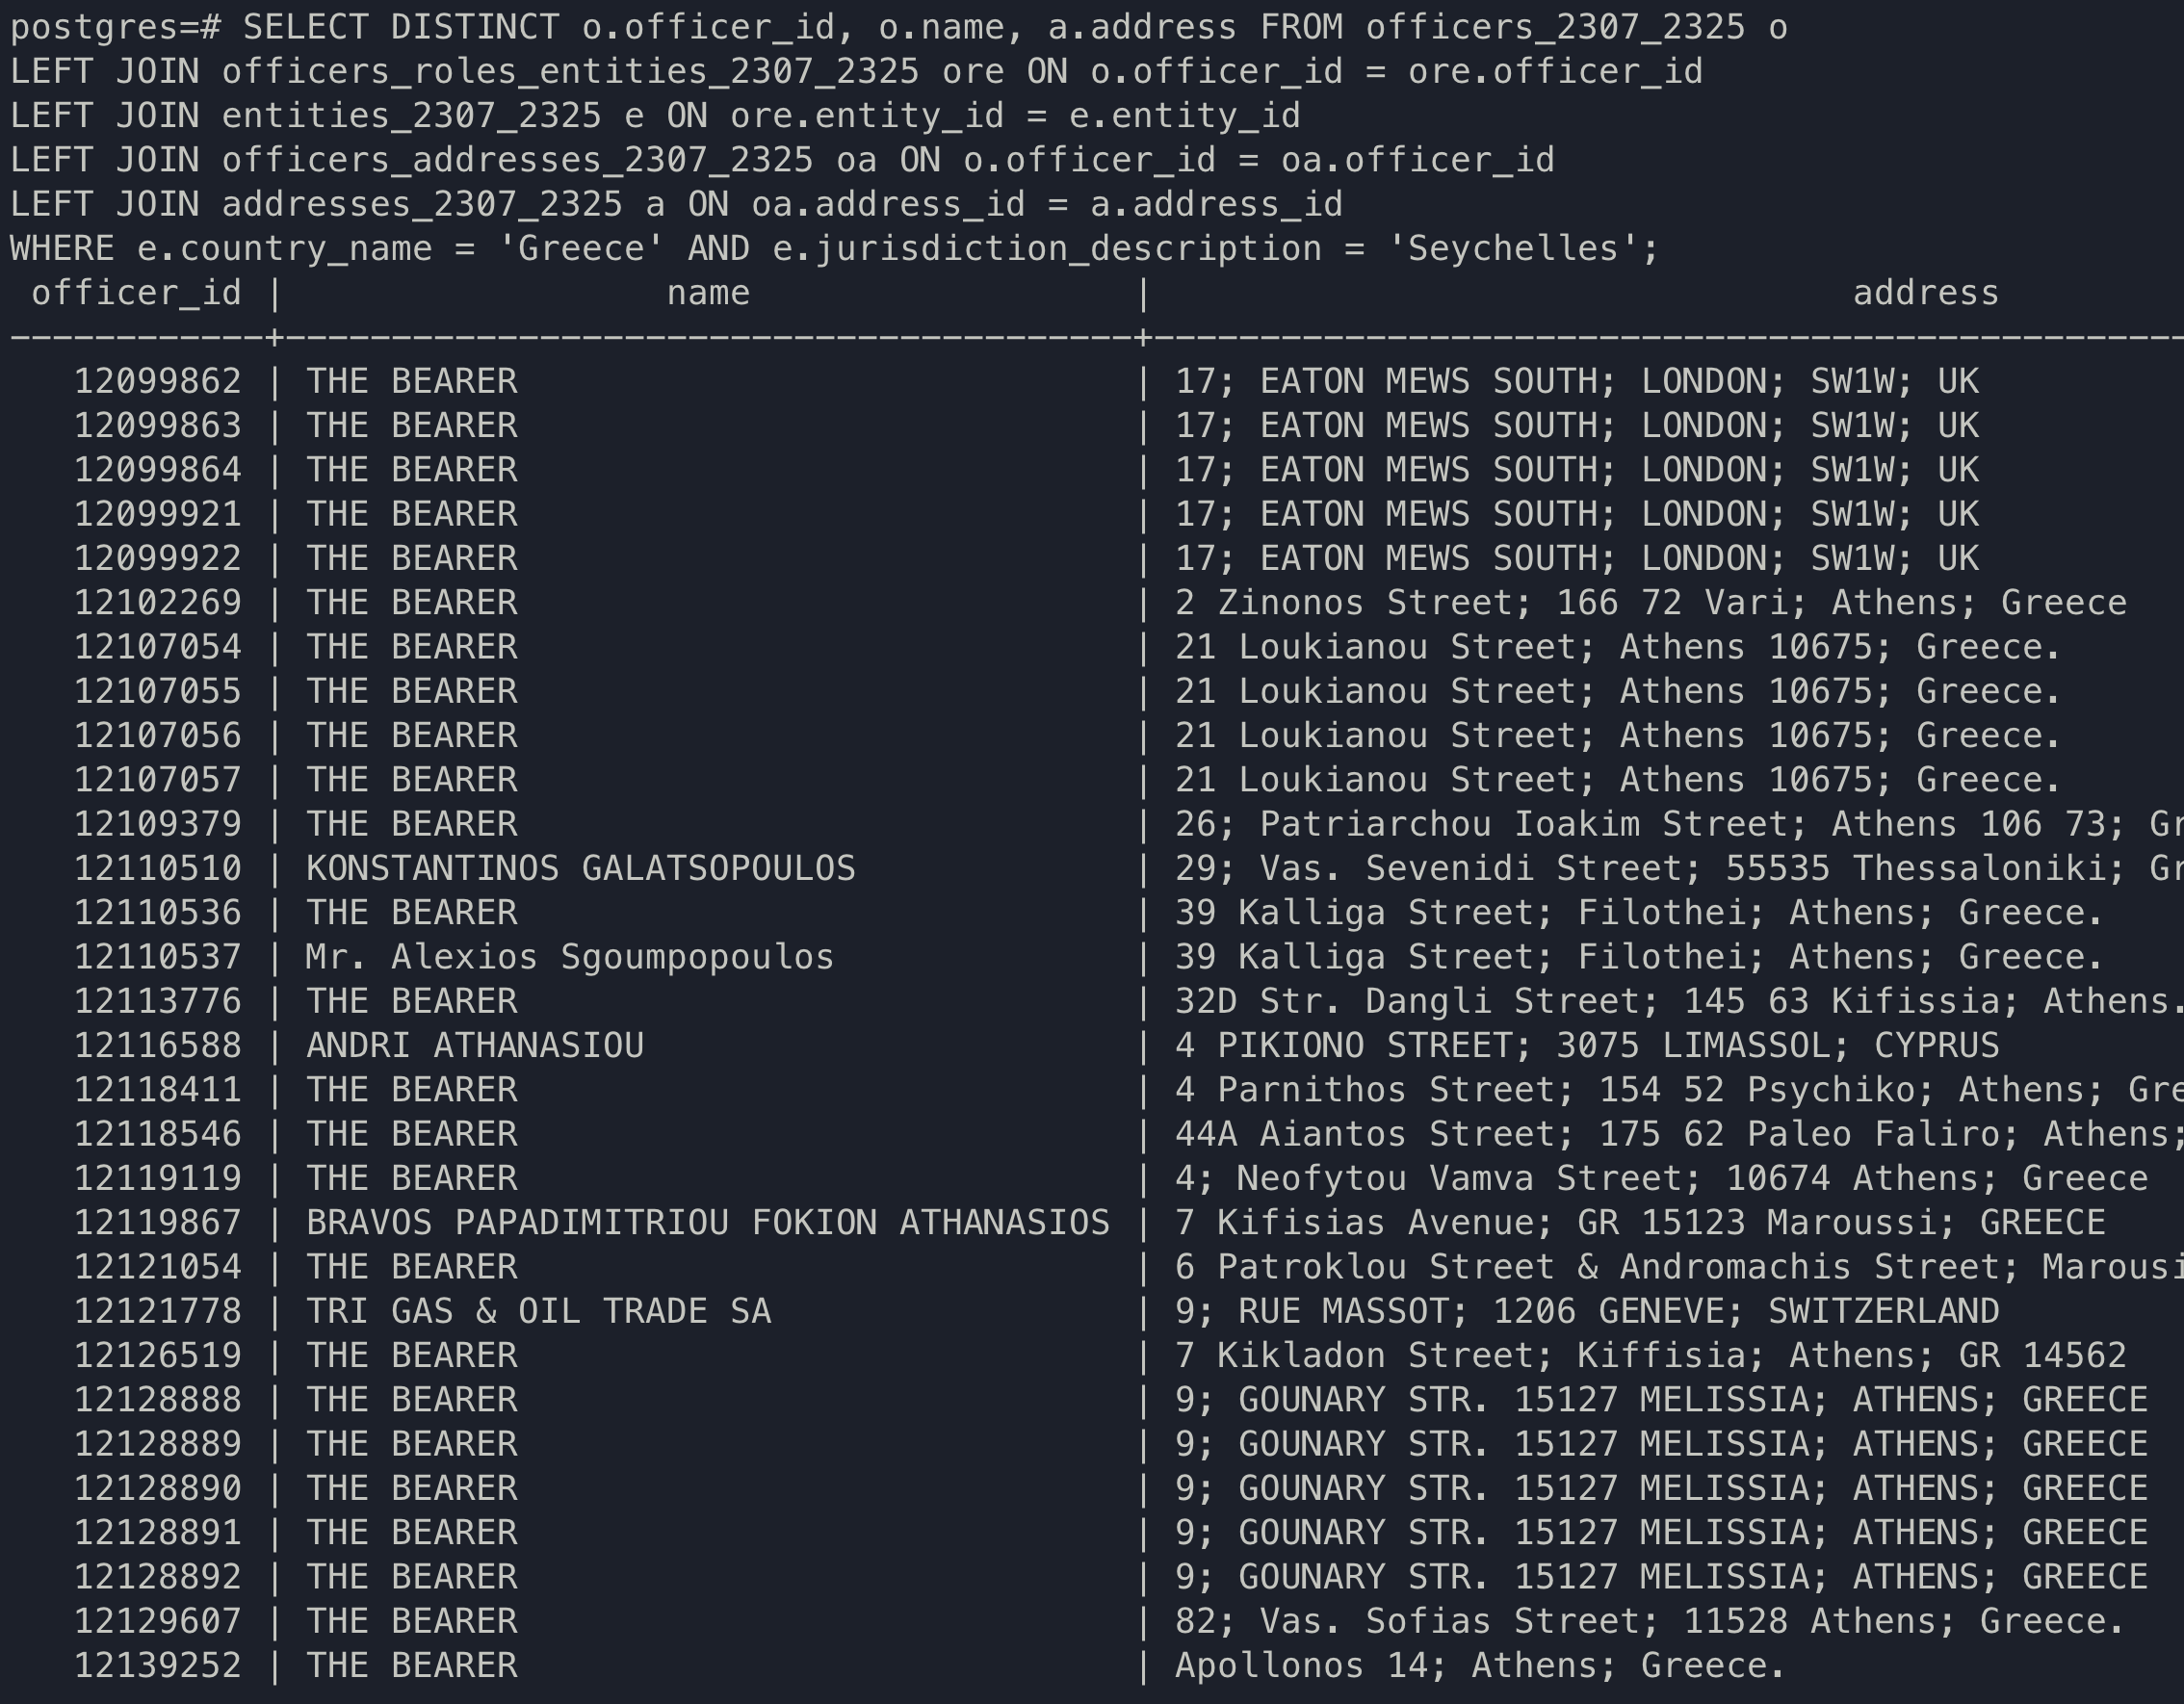
\includegraphics[width=0.9\linewidth]{Q4.png}
    \captionsetup{labelformat=empty}
    \caption{Question 4}
\end{figure}



\newpage
\section*{Question v}
Modify an officer’s address by removing all previous addresses and inserting a new one (of your selection).

\begin{figure}[h]
    \centering
    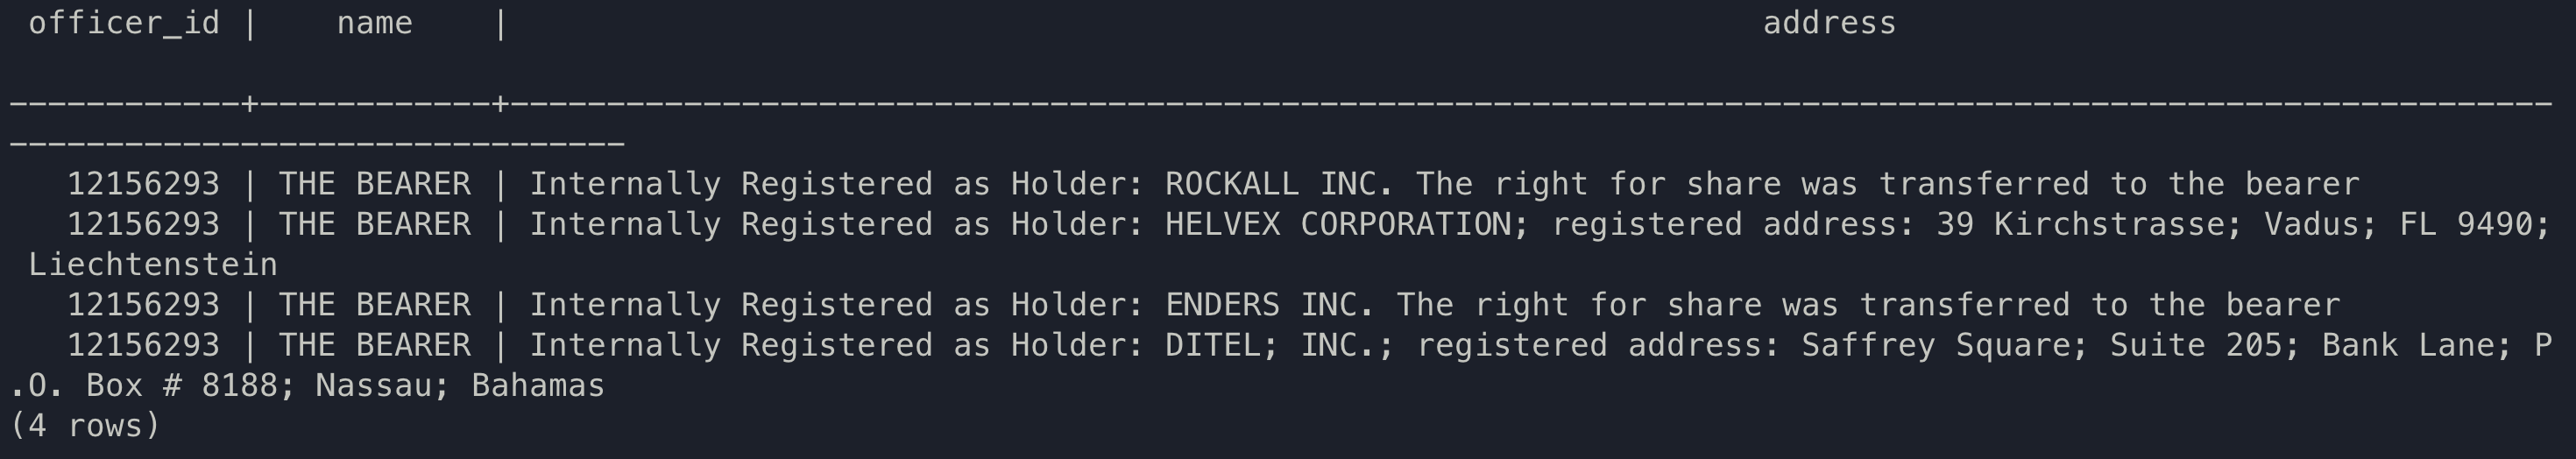
\includegraphics[width=0.9\linewidth]{Q5b.png}
    \captionsetup{labelformat=empty}
    \caption{Question 5: Selecting the officer's address to be modified.}
\end{figure}

\begin{figure}[h]
    \centering
    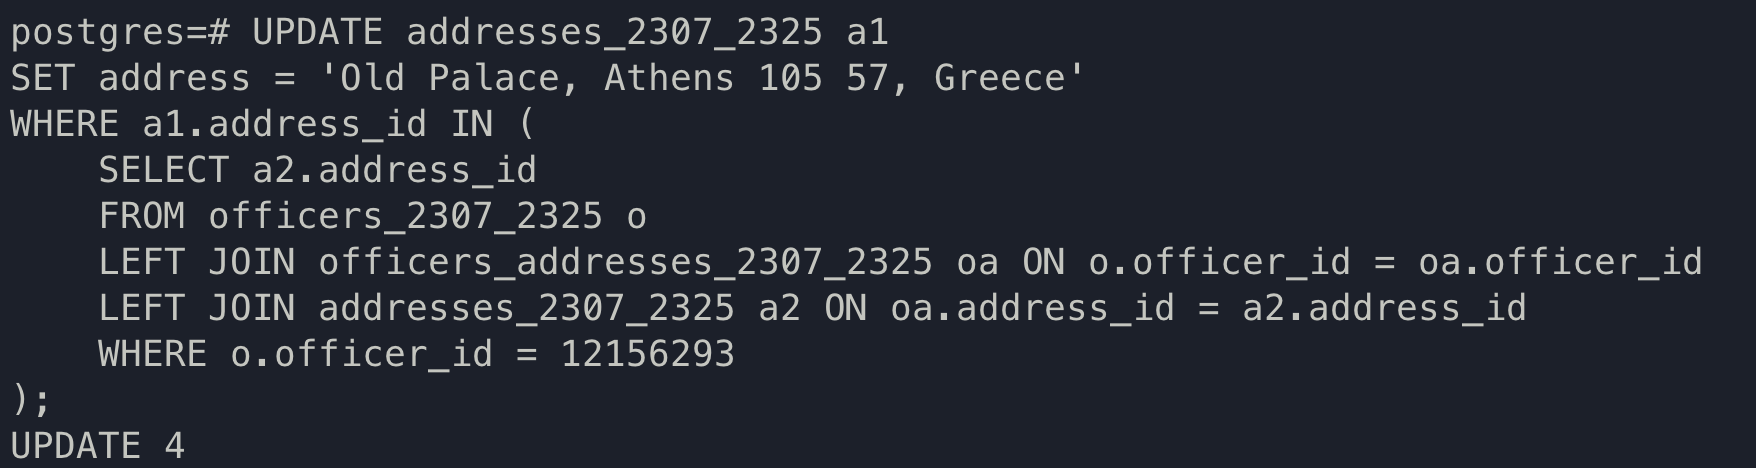
\includegraphics[width=0.9\linewidth]{Q5c.png}
    \captionsetup{labelformat=empty}
    \caption{Question 5: Update the address.}
\end{figure}

\begin{figure}[h]
    \centering
    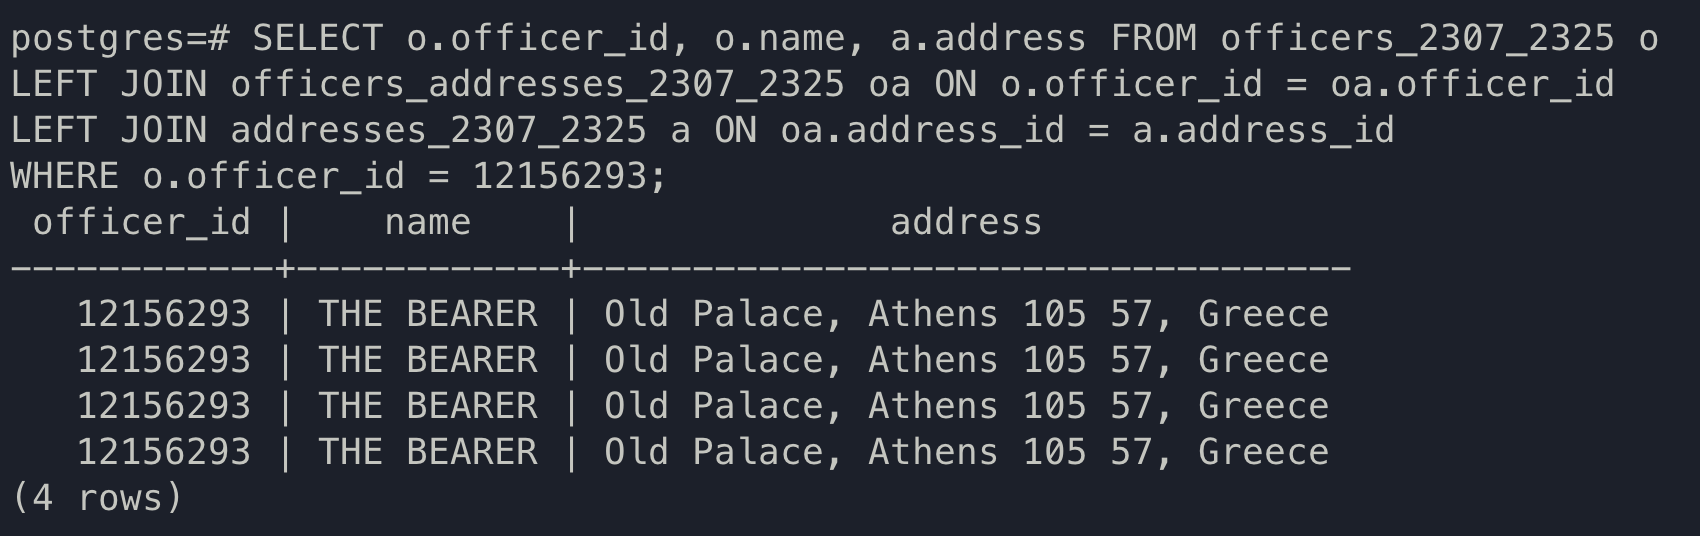
\includegraphics[width=0.9\linewidth]{Q5d.png}
    \captionsetup{labelformat=empty}
    \caption{Question 5: Selecting the officer's address to see the modification.}
\end{figure}

\end{document}
